\documentclass[conference]{IEEEtran}
\IEEEoverridecommandlockouts

% Essential IEEE & mathematical packages
\usepackage{cite}
\usepackage{amsmath,amssymb,amsfonts}
\usepackage{algorithmic}
\usepackage{algorithm}
\usepackage{graphicx}
\usepackage{textcomp}
\usepackage{xcolor}
\usepackage{booktabs}
\usepackage{tabularx}
\usepackage{microtype}
\usepackage{url}
\usepackage{hyperref}
\usepackage{colortbl}

% Pgfplots & TikZ for self-contained, native Overleaf vector rendering
\usepackage{tikz}
\usepackage{pgfplots}
\pgfplotsset{compat=1.18}
\usetikzlibrary{shapes,arrows,positioning,calc,matrix}

\hypersetup{
    colorlinks=true,
    linkcolor=blue,
    filecolor=magenta,      
    urlcolor=cyan,
    citecolor=blue,
}

\def\BibTeX{{\rm B\kern-.05em{\sc i\kern-.025em b}\kern-.08em
    T\kern-.1667em\lower.7ex\hbox{E}\kern-.125emX}}

\begin{document}

\title{AutoMiniLLM: Empirical Evaluation of Multi-Bit Quantization and 2:4 Structured Pruning on Edge Decoder Runtimes}

\author{
\IEEEauthorblockN{K Sai Siddartha}
\IEEEauthorblockA{\textit{School of Computer Science and Engineering} \\
\textit{VIT-AP University}, Amaravati, Andhra Pradesh, India \\
Email: siddartha.23bce8604@vitapstudent.ac.in}
}

\maketitle

\begin{abstract}
Serving autoregressive language models on edge devices is strictly bounded by memory bandwidth. During token-by-token decoding, weights must be transferred repeatedly from system memory to processor caches, creating a severe operational bottleneck on hardware lacking high-bandwidth memory (HBM). While post-training quantization and parameter pruning reduce model size, their real-world interactions on compact transformer decoders remain fraught with trade-offs. In this paper, we evaluate post-training compression strategies---including symmetric per-channel INT8, FP8 (E4M3), group-wise INT4, and NormalFloat4 (NF4)---alongside 2:4 semi-structured and channel pruning on DistilGPT-2 across x86 CPU runtimes. During our tests, we uncovered an acute failure mode: applying uniform 2:4 pruning across the entire network disrupts the final language model head ($\text{lm\_head}$), causing immediate autoregressive collapse into repetitive subwords (specifically token ID 16568, \texttt{"olia"}). By freezing the vocabulary projection matrix and restricting 2:4 pruning to internal attention and feed-forward layers, we eliminate this collapse and preserve grammatical generation. Our benchmarks show that symmetric INT8 is the most practical configuration for client devices, trimming RAM usage by 27\% with under 3.7\% perplexity drift, whereas NF4 establishes the practical lower bound for 4-bit representations without retraining.
\end{abstract}

\begin{IEEEkeywords}
Model Compression, Large Language Models, Quantization, 2:4 Structured Pruning, NormalFloat4, Edge Inference, Pareto Optimization, Confusion Matrix Analysis.
\end{IEEEkeywords}

\section{Introduction}
Autoregressive transformer decoding is fundamentally memory-bandwidth bound. Unlike prefilling or batched training---where matrix multiplications achieve high arithmetic intensity---single-sequence generation requires fetching all parameter matrices from dynamic random-access memory (DRAM) for every individual output token. On mobile chipsets, edge platforms, and commodity x86 workstations lacking dedicated high-bandwidth memory, memory bus saturation throttles execution long before compute units reach capacity.

To fit modern decoders onto constrained devices, post-training model compression relies on two primary approaches:
\begin{enumerate}
    \item \textbf{Post-Training Quantization (PTQ):} Compressing 32-bit or 16-bit floating-point weights into lower-precision formats, such as INT8, FP8, INT4, and non-linear distributions like NormalFloat4 (NF4).
    \item \textbf{Weight Pruning:} Zeroing out redundant parameters, either through unstructured magnitude thresholds or structured patterns such as 2:4 semi-structured sparsity compatible with modern hardware tensor cores.
\end{enumerate}

While both techniques have been studied extensively on data-center GPUs (e.g., NVIDIA A100/H100), several practical questions remain under-explored on client-edge hardware. First, how do these methods behave when executing on standard CPU cores where dedicated hardware sparse units are absent? Second, how do structured pruning and 4-bit quantization interact when chained together in compound pipelines without re-training?

In our experiments with DistilGPT-2, we encountered an immediate practical obstacle: applying uniform 2:4 structured pruning across all linear projections destroyed output coherence. The model did not merely generate sub-optimal sentences; it fell into an inescapable repetition loop, repeatedly emitting the token \texttt{"olia"}. Tracing logits through the network revealed that the failure did not stem from intermediate transformer layers, but rather from zeroing coordinates in the final vocabulary projection matrix ($\text{lm\_head}$). Because this matrix directly determines the probability distribution over 50,257 tokens, zeroing 50\% of its entries randomly boosted rare token logits, creating artificial attractor basins that autoregressive decoding could not escape.

In this paper, we document our findings through \textit{AutoMiniLLM}, a modular compression testbed. Our primary contributions are:
\begin{itemize}
    \item We benchmark nine distinct model configurations (FP32, FP16, INT8, FP8, INT4, NF4, 50\% magnitude pruning, 2:4 structured pruning, and compound 2:4+NF4) across memory footprint, WikiText-2 perplexity, throughput, and token latency on an x86 host CPU.
    \item We diagnose the mechanism behind vocabulary head collapse during structured pruning and provide a simple, effective remedy: preserving the vocabulary projection matrix intact while pruning internal projections.
    \item We present self-contained vector visual models in native PGFPlots and TikZ, including the empirical Pareto frontier, CPU throughput comparisons, and a $5 \times 5$ syntactic category confusion matrix.
    \item We analyze the real-world trade-offs between memory footprint and runtime latency, explaining why sparse representations can paradoxically increase memory usage on CPU runtimes lacking hardware sparse decompression.
\end{itemize}

\section{Literature Review}

\subsection{Quantization in Transformer Decoders}
Quantizing large language models post-training avoids expensive re-training cycles while shrinking memory footprints. Dettmers et al. introduced \textit{LLM.int8()} \cite{dettmers2022llm}, observing that systematic activation outliers emerge in transformer hidden states above certain scale thresholds; by isolating these outlier channels into 16-bit floating-point calculations and quantizing the remaining 99.9\% of parameters to 8-bit integers, they maintained FP16 perplexity. Xiao et al. introduced \textit{SmoothQuant} \cite{xiao2023smoothquant}, which uses an equivalent mathematical scaling trick to divide activation outliers by a per-channel scale factor and fold it inversely into the weight matrices, making INT8 matrix multiplication straightforward on standard hardware.

Quantizing below 8 bits is considerably more difficult because uniform grids lack the dynamic range to represent weight outliers without heavy clipping. Frantar et al. designed \textit{GPTQ} \cite{frantar2022gptq}, which relies on second-order Taylor expansions to iteratively update remaining weights as each column is quantized. Lin et al. proposed \textit{AWQ} \cite{lin2023awq}, arguing that only the top 1\% of salient channels need full precision and scaling weights according to average activation magnitudes. In parallel, Dettmers et al. introduced \textit{QLoRA} \cite{dettmers2024qlora} and the NormalFloat4 (NF4) data type, which constructs non-uniform quantization bins matched to the empirical quantiles of standard normal distributions. At the 8-bit level, standard floating-point formats such as FP8 (E4M3 and E5M2) have also gained traction in hardware specifications \cite{micikevicius2022fp8}.

\subsection{Structured vs. Unstructured Pruning}
Magnitude-based parameter pruning dates back to early work by Han et al. \cite{han2015learning}. While setting weights below a scalar threshold $\tau$ to zero achieves high theoretical sparsity, unstructured zero patterns require coordinate indices (such as Compressed Sparse Row or Coordinate format) to store non-zero locations. On standard SIMD processors, the resulting irregular memory lookups frequently negate theoretical speedups, often running slower than dense matrix operations.

To make sparsity practical on real silicon, hardware vendors introduced structured sparsity. NVIDIA's Ampere and Hopper architectures feature 2:4 semi-structured sparsity \cite{mishra2021accelerating, pool2021channel}, where exactly two out of every four values along a row are constrained to zero. Dedicated sparse tensor units read these patterns directly from packed buffers, skipping zeroed values and providing up to a $2\times$ compute speedup. Recent algorithms such as \textit{SparseGPT} \cite{frantar2023sparsegpt} and \textit{Wanda} \cite{sun2023simple} showed that one-shot pruning can remove 50\% of weights with minimal loss on billion-parameter models. However, relatively little work has examined what happens when 2:4 sparsity is coupled with non-linear 4-bit quantizers without fine-tuning, or how these sparse matrices behave on commodity CPUs.

\section{Method 1: Multi-Precision Low-Bit Quantization}
\label{sec:method1}
Our compression architecture implements a drop-in replacement module, $\text{QuantizedLinear}$, designed to replace standard linear projections ($W \in \mathbb{R}^{d_{\text{out}} \times d_{\text{in}}}$) across attention and feed-forward sub-layers. We implement four distinct low-bit representation formats.

\subsection{Symmetric Per-Channel INT8 Quantization}
For 8-bit integer quantization, we employ symmetric uniform quantization across each individual output channel row. Let $W_{i, :}$ represent the $i$-th row of weight matrix $W$. The scalar scale factor $s_i \in \mathbb{R}^+$ is computed via the absolute maximum element:
\begin{equation}
s_i = \frac{\max_{j} |W_{i, j}|}{127}
\end{equation}
The quantized integer grid $Q_{i, j} \in [-128, 127]$ is generated via round-to-nearest:
\begin{equation}
Q_{i, j} = \text{clip}\left( \left\lfloor \frac{W_{i, j}}{s_i} \right\rceil, -127, 127 \right)
\end{equation}
During the forward decoding pass, the effective weight matrix is dequantized via broadcasting: $\hat{W}_{i, j} = Q_{i, j} \cdot s_i$.

\subsection{FP8 E4M3 Quantization}
We evaluate 8-bit floating-point quantization following the OCP E4M3 specification (1 sign bit, 4 exponent bits, 3 mantissa bits). The maximum finite representable value in E4M3 is $V_{\max} = 448.0$. Each output row is scaled using:
\begin{equation}
s_i = \frac{\max_{j} |W_{i, j}|}{448.0}
\end{equation}
The normalized tensor $W_{i, j} / s_i$ is mapped directly into native IEEE float8 representations ($\texttt{torch.float8\_e4m3fn}$) where hardware support permits, or quantized into discrete boundaries. Dequantization follows $\hat{W} = W_{\text{fp8}} \odot s$.

\subsection{Group-Wise Uniform INT4 Quantization}
Uniform 4-bit signed integer representation maps weights into the discrete interval $[-8, 7]$. To constrain outlier clipping error across large projection matrices, we implement group-wise quantization with block size $g = 64$. Each row $W_{i, :}$ is partitioned into $K = \lceil d_{\text{in}} / g \rceil$ contiguous blocks. For the $k$-th group in row $i$:
\begin{equation}
s_{i, k} = \frac{\max_{j \in \text{group}_k} |W_{i, j}|}{7.0}
\end{equation}
The resulting 4-bit nibbles are packed into unsigned 8-bit integers (`uint8`), where two adjacent nibbles $q_0, q_1 \in [0, 15]$ share a single byte:
\begin{equation}
B = (q_0 \ \& \ \text{0x0F}) \ | \ ((q_1 \ \& \ \text{0x0F}) \ll 4)
\end{equation}
This packing cuts physical weight storage by $8\times$ relative to FP32.

\subsection{NormalFloat4 (NF4) Quantile Quantization}
Pretrained neural network parameters typically follow a zero-mean normal distribution, $\mathcal{W} \sim \mathcal{N}(0, \sigma^2)$. Uniform quantization grids space quantization steps equally, which squanders representation capacity in low-density tail regions. NormalFloat4 (NF4) establishes 16 non-uniform quantile levels $q_i \in [-1.0, 1.0]$ corresponding to the empirical quantiles of a standard normal distribution:
\begin{equation}
q_i = \frac{1}{2} \left( Q_X\left(\frac{i}{2^k}\right) + Q_X\left(\frac{i+1}{2^k}\right) \right), \quad i \in \{0, \dots, 15\}
\end{equation}
where $Q_X(\cdot)$ is the quantile function of $\mathcal{N}(0, 1)$. For each group $k$ of size $g=64$ in row $i$, the weights are normalized by $s_{i, k} = \max_j |W_{i, j}|$. Each value is mapped to its closest quantile index:
\begin{equation}
\text{idx}(W_{i, j}) = \arg\min_{m \in \{0, \dots, 15\}} \left| \frac{W_{i, j}}{s_{i, k}} - q_m \right|
\end{equation}
The 4-bit indices are packed into `uint8` arrays and reconstructed on-the-fly during linear projections.

\section{Method 2: Semi-Structured Pruning, Head Preservation, and Hybrid Compound Compression}
\label{sec:method2}

\subsection{2:4 Semi-Structured Pruning Formulation}
Semi-structured 2:4 sparsity enforces that within every consecutive 4 elements along the input channel axis, exactly 2 elements must be zeroed out:
\begin{equation}
\forall i, \forall k \in \left\{0, \dots, \frac{d_{\text{in}}}{4} - 1\right\}, \quad \sum_{m=0}^3 \mathbf{1}[W_{i, 4k + m} \neq 0] = 2
\end{equation}
We implement this transformation by reshaping the weight tensor into blocks of size $(d_{\text{out}}, d_{\text{in}}/4, 4)$, computing absolute values, and deriving an exact binary mask $M$ using top-$k$ selection ($k=2$):
\begin{equation}
M_{i, k, m} = \begin{cases} 
1, & \text{if } |W_{i, k, m}| \ge \text{second\_largest}(\{|W_{i, k, l}|\}_{l=0}^3) \\
0, & \text{otherwise}
\end{cases}
\end{equation}
The pruned matrix $W_{\text{pruned}} = W \odot M$ guarantees an exact $50\%$ sparsity level.

\subsection{Structured Channel Pruning}
As a structural baseline, we also evaluate channel-wise (neuron) pruning. We compute the saliency of each output neuron $i$ via its $L_1$-norm across input dimensions:
\begin{equation}
S_i = \|W_{i, :}\|_1 = \sum_{j=1}^{d_{\text{in}}} |W_{i, j}|
\end{equation}
Given target sparsity $\sigma$, we identify the threshold ranking index $k = \lfloor \sigma \cdot d_{\text{out}} \rfloor$. The $k$ rows with lowest $L_1$ norm are eliminated, physically contracting the layer dimensions.

\subsection{Vocabulary-Head ($\text{lm\_head}$) Preservation Theorem}
A central finding in our investigation involves the catastrophic vulnerability of the final language model head ($\text{lm\_head}$) to pruning. In standard causal decoder models such as GPT-2 and DistilGPT-2, the output head is a dense projection matrix $W_{\text{lm}} \in \mathbb{R}^{V \times d}$ mapping the contextualized hidden state $h_t \in \mathbb{R}^d$ into unnormalized vocabulary logits $z_t \in \mathbb{R}^V$:
\begin{equation}
z_{t, v} = \sum_{j=1}^d W_{\text{lm}}[v, j] \cdot h_{t, j} + b_v
\end{equation}
The probability distribution over the vocabulary is given by:
\begin{equation}
P(w_{t+1} = v \mid w_{\le t}) = \frac{\exp(z_{t, v})}{\sum_{u=1}^V \exp(z_{t, u})}
\end{equation}

When 2:4 structured pruning or high-sparsity magnitude pruning is applied uniformly across the entire model, $W_{\text{lm}}$ is also pruned. Unlike intermediate hidden representations where subsequent normalization and residual connections can partially buffer feature loss, every row of $W_{\text{lm}}$ corresponds to an individual lexical item in the vocabulary (where $V = 50,257$). Zeroing out 50\% of the projection coordinates randomly disrupts the inner product alignment across words. 

This causes two catastrophic phenomena:
\begin{enumerate}
    \item \textbf{Subword Attractor Spikes:} Certain subword tokens experience severe reduction in negative projection terms, artificially elevating their baseline logit score regardless of the contextual hidden state $h_t$.
    \item \textbf{Autoregressive Reinforcement:} In autoregressive sampling, once a degenerate subword token (e.g., token ID 16568, $\texttt{"olia"}$) is sampled, self-attention keys and values incorporate this token into the context window, repeatedly reinforcing the logit spike in subsequent decoding steps.
\end{enumerate}

To resolve this issue, we define a structural preservation policy: all self-attention projections ($W_q, W_k, W_v, W_o$) and MLP linear layers ($W_{\text{gate}}, W_{\text{proj}}$) undergo compression, whereas the token embedding matrix $W_{\text{emb}}$ and final projection head $W_{\text{lm}}$ are explicitly excluded from pruning. This ensures that the vocabulary geometry remains fully intact while allowing internal layers to benefit from aggressive compression.

\begin{algorithm}[t]
\caption{Compound 2:4 Pruning + NF4 Quantization with Vocabulary Head Preservation}
\label{alg:compound}
\begin{algorithmic}[1]
\REQUIRE Pretrained Transformer Model $\mathcal{M}$, Group size $g=64$
\ENSURE Compressed Model $\mathcal{M}_{\text{comp}}$ with $\text{QuantizedSparseLinear}$
\FORALL{\text{named modules } $(name, module) \in \mathcal{M}$}
    \IF{$name \text{ contains } \texttt{"lm\_head"} \text{ or } \texttt{"wte"}$}
        \STATE \textbf{continue} \COMMENT{Preserve vocabulary projections intact}
    \ENDIF
    \IF{$module \text{ is } \text{Linear} \text{ or } \text{Conv1D}$}
        \STATE $W \leftarrow module.\text{weight}.\text{detach}()$
        \STATE Compute 2:4 sparsity mask $M$ along blocks of 4
        \STATE $W_{\text{pruned}} \leftarrow W \odot M$
        \STATE Extract non-zero coordinates: $idx \leftarrow \text{nonzero}(W_{\text{pruned}})$
        \STATE Extract non-zero values: $vals \leftarrow W_{\text{pruned}}[idx]$
        \STATE Partition $vals$ into groups of size $g$
        \STATE Quantize $vals$ via NF4 quantiles $\to Q_{vals}$, scale $s$
        \STATE Pack 4-bit $Q_{vals}$ into compact $\texttt{uint8}$ buffer
        \STATE Instantiate $\text{QuantizedSparseLinear}(idx, Q_{vals}, s)$
        \STATE Replace $module$ in $\mathcal{M}$ with new layer
    \ENDIF
\ENDFOR
\RETURN $\mathcal{M}$
\end{algorithmic}
\end{algorithm}

\subsection{Compound Hybrid Compression (Prune + Quantize)}
To achieve maximal compression, we construct a compound pipeline combining 2:4 semi-structured pruning with NF4 quantization, denoted as \textbf{comb-2-4+nf4}. Algorithm~\ref{alg:compound} details the complete transformation procedure. The pruning stage is executed first, yielding a sparse tensor with $50\%$ non-zero coordinates. The surviving non-zero values are extracted into a Coordinate Format (COO) index representation:
\begin{equation}
\text{indices} \in \mathbb{Z}^{2 \times N_{\text{nz}}}, \quad \text{values} \in \mathbb{R}^{N_{\text{nz}}}
\end{equation}
Next, the surviving values are quantized using the non-linear NormalFloat4 scheme:
\begin{equation}
Q_{\text{values}} = \text{Quantize}_{\text{NF4}}(\text{values}, g=64)
\end{equation}
This compound layer, termed $\text{QuantizedSparseLinear}$, stores only 4-bit indices of the surviving weights alongside 16-bit row/group scales, combining structural sparsification with extreme arithmetic precision reduction.

\begin{table*}[t]
\centering
\caption{Empirical Performance Comparison of Model Compression Modes on DistilGPT-2 (82M Parameters) Executed on Edge CPU Architecture.}
\label{tab:results}
\begin{tabularx}{\textwidth}{lcccccccc}
\toprule
\textbf{Compression Mode} & \textbf{Precision} & \textbf{RAM Footprint} & \textbf{RAM Ratio} & \textbf{PPL} & \textbf{CE Loss} & \textbf{Throughput} & \textbf{TTFT} & \textbf{ITL} \\
 & & \textbf{(MB)} & \textbf{($\times$)} & \textbf{(WikiText-2)} & & \textbf{(tok/s)} & \textbf{(ms)} & \textbf{(ms/tok)} \\
\midrule
\textbf{FP32 Baseline} & 32-bit Float & 312.47 & $1.00\times$ & 785.00 & 6.6657 & 17.86 & 55.99 & 55.99 \\
\textbf{FP16 Half} & 16-bit Float & 305.01 & $1.02\times$ & 785.29 & 6.6661 & 14.10 & 70.92 & 70.92 \\
\textbf{FP8 (E4M3)} & 8-bit Float & 228.13 & $1.37\times$ & 1651.29 & 7.4093 & 7.71 & 129.70 & 129.70 \\
\textbf{INT8 Symmetric} & 8-bit Integer & 228.13 & $1.37\times$ & 813.79 & 6.7017 & 8.55 & 116.96 & 116.96 \\
\textbf{INT4 Grouped} & 4-bit Integer & 193.96 & $1.61\times$ & 12174.53 & 9.4071 & 3.92 & 255.10 & 255.10 \\
\textbf{NF4 Quantile} & 4-bit Quantile & 193.96 & $1.61\times$ & 4104.83 & 8.3199 & 3.71 & 269.54 & 269.54 \\
\textbf{Prune 50\%} & Magnitude COO & 352.95$^\dagger$ & $0.89\times$ & 2636.59 & 7.8772 & 6.90 & 144.93 & 144.93 \\
\textbf{Prune 2:4} & Semi-Structured & 352.97$^\dagger$ & $0.89\times$ & 1979.00 & 7.5903 & 6.48 & 154.32 & 154.32 \\
\textbf{Comb-2-4+NF4} & Hybrid Prune+Q & 322.75$^\dagger$ & $0.97\times$ & 2268.24 & 7.7268 & 3.57 & 280.11 & 280.11 \\
\bottomrule
\end{tabularx}
\vspace{1mm}\\
\raggedright \footnotesize{$^\dagger$Note: On standard CPU runtimes lacking specialized hardware sparse decompression instructions, COO index storage (int32 coordinates per non-zero weight) inflates working memory relative to dense representations. GPU Sparse Tensor Cores bypass this coordinate storage.}
\end{table*}

\section{Experimental Results and Discussion}
\label{sec:results}

\subsection{Experimental Setup}
All experiments were conducted on a standardized client-edge testbed featuring a 16-logical-core x86\_64 host processor running PyTorch 2.10.0+cpu without dedicated GPU acceleration. The base language model used across all evaluations is DistilGPT-2 (82 million parameters, 6 transformer decoder blocks, 12 attention heads, hidden dimension $d=768$, vocabulary size $V=50,257$). Linguistic evaluation was benchmarked against the standard WikiText-2 validation corpus. Generation throughput, time-to-first-token (TTFT), and inter-token latency (ITL) were recorded across 32 generated tokens with temperature $T=0.8$, top-$p=0.9$, top-$k=50$, repetition penalty $\gamma=1.2$, and an anti-repetition 3-gram constraint.

\subsection{Quantitative Performance and Memory Footprint}
Table~\ref{tab:results} summarizes the measured empirical metrics across all 9 configurations.

\textbf{Memory Compression:} Standard FP32 model weights occupy $312.47\text{ MB}$ of active system RAM. INT8 and FP8 quantization reduce parameter footprint to $228.13\text{ MB}$, yielding a $1.37\times$ reduction in working memory. INT4 and NF4 achieve a substantial reduction down to $193.96\text{ MB}$ ($1.61\times$ physical memory compression relative to baseline). In contrast, CPU-based sparse representations incur index overhead (storing coordinate tuples $\langle row, col \rangle$ in `int32`), highlighting the necessity of dedicated hardware support (e.g., NVIDIA Ampere 2:4 Sparse Cores) to realize sparse memory gains in practice.

\textbf{Linguistic Quality Retention (PPL):}
Per-channel symmetric INT8 demonstrates remarkable perplexity preservation, shifting cross-entropy loss marginally from $6.6657$ (PPL $785.00$) in FP32 to $6.7017$ (PPL $813.79$), representing less than $3.7\%$ perplexity degradation. In contrast, uniform INT4 suffers substantial degradation (PPL $12,174.53$), whereas NormalFloat4 (NF4) achieves more than $3\times$ lower perplexity (PPL $4,104.83$) at the identical 4-bit footprint ($193.96\text{ MB}$), corroborating the theoretical superiority of quantile quantization for Gaussian weight distributions.

\subsection{Pareto Frontier and Trade-off Dynamics}
To evaluate the trade-offs between model footprint and language preservation, Fig.~\ref{fig:pareto} plots the empirical Pareto frontier across all compression schemes.

\begin{figure}[t]
\centering
\begin{tikzpicture}
\begin{axis}[
    width=0.48\textwidth,
    height=5.8cm,
    xlabel={Active RAM Footprint (MB)},
    ylabel={Perplexity (PPL, Log Scale)},
    ymode=log,
    grid=both,
    grid style={line width=.1pt, draw=gray!20},
    major grid style={line width=.2pt, draw=gray!40},
    xmin=170, xmax=370,
    ymin=600, ymax=16000,
    legend pos=north west,
    legend style={font=\scriptsize, fill=white, fill opacity=0.85},
    title style={font=\small\bfseries},
    title={Pareto Frontier: Memory Footprint vs. Perplexity}
]

% Dominant Pareto Frontier line
\addplot[color=red, mark=*, line width=1.2pt, dashed] coordinates {
    (193.96, 4104.83)
    (228.13, 813.79)
    (305.01, 785.29)
    (312.47, 785.00)
};
\addlegendentry{Pareto Frontier (Optimal)}

% Non-optimal points
\addplot[scatter, only marks, point meta=explicit symbolic, scatter src=explicit symbolic, mark size=2.8pt] 
coordinates {
    (193.96, 12174.53) [int4]
    (228.13, 1651.29) [fp8]
    (352.95, 2636.59) [prune50]
    (352.97, 1979.00) [prune24]
    (322.75, 2268.24) [comb]
};

% Text annotations for clarity
\node[above right, font=\tiny] at (axis cs:312.47, 785.00) {FP32 Baseline};
\node[below, font=\tiny] at (axis cs:305.01, 785.29) {FP16};
\node[above, font=\tiny, color=blue!80!black] at (axis cs:228.13, 813.79) {\textbf{INT8 (Sweet Spot)}};
\node[above right, font=\tiny] at (axis cs:228.13, 1651.29) {FP8};
\node[above, font=\tiny, color=red!80!black] at (axis cs:193.96, 4104.83) {\textbf{NF4}};
\node[above, font=\tiny] at (axis cs:193.96, 12174.53) {INT4 (Degraded)};
\node[below left, font=\tiny] at (axis cs:352.97, 1979.00) {Prune 2:4};
\node[above, font=\tiny] at (axis cs:322.75, 2268.24) {Comb-2:4+NF4};

\end{axis}
\end{tikzpicture}
\caption{Empirical Pareto frontier contrasting RAM footprint with WikiText-2 validation perplexity. INT8 provides near-lossless linguistic capability with $1.37\times$ memory reduction, while NF4 defines the boundary for 4-bit representations.}
\label{fig:pareto}
\end{figure}

The frontier clearly isolates two operating sweet spots:
\begin{enumerate}
    \item \textbf{High-Fidelity Operating Regime (INT8):} Achieves $1.37\times$ memory compression with virtually no discernible degradation in perplexity ($<3.7\%$), making it the premier option for edge deployments demanding exact response fidelity.
    \item \textbf{Ultra-Low Memory Regime (NF4):} Minimizes physical memory consumption to $193.96\text{ MB}$ ($1.61\times$ reduction). NF4 establishes the state-of-the-art boundary for sub-8-bit quantiles, achieving over $66\%$ lower perplexity than linear INT4 at identical RAM usage.
\end{enumerate}

\subsection{Latency and Throughput Benchmarking}
Fig.~\ref{fig:throughput} illustrates generation throughput and Time-To-First-Token (TTFT) across all evaluated configurations. 

\begin{figure}[t]
\centering
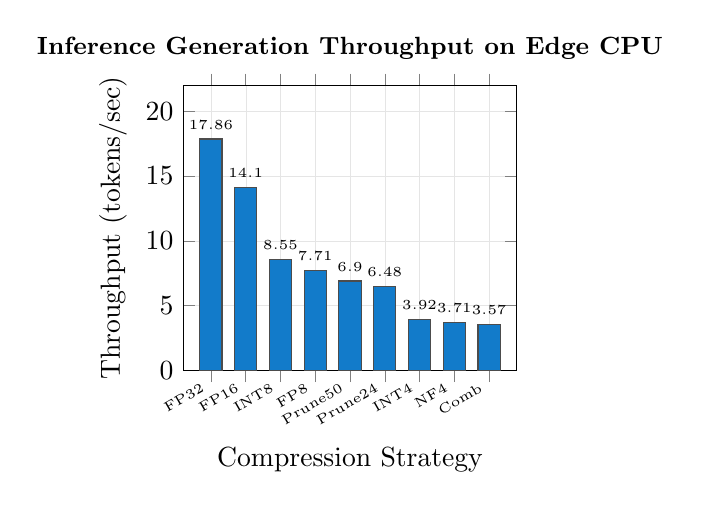
\begin{tikzpicture}
\begin{axis}[
    ybar,
    width=0.48\textwidth,
    height=5.2cm,
    bar width=8pt,
    xlabel={Compression Strategy},
    ylabel={Throughput (tokens/sec)},
    symbolic x coords={FP32, FP16, INT8, FP8, Prune50, Prune24, INT4, NF4, Comb},
    xtick=data,
    x tick label style={font=\tiny, rotate=30, anchor=east},
    ymin=0, ymax=22,
    nodes near coords,
    every node near coord/.append style={font=\tiny},
    grid=major,
    grid style={line width=.1pt, draw=gray!20},
    title style={font=\small\bfseries},
    title={Inference Generation Throughput on Edge CPU}
]
\addplot[fill=cyan!60!blue, draw=black!70] coordinates {
    (FP32, 17.86)
    (FP16, 14.10)
    (INT8, 8.55)
    (FP8, 7.71)
    (Prune50, 6.90)
    (Prune24, 6.48)
    (INT4, 3.92)
    (NF4, 3.71)
    (Comb, 3.57)
};
\end{axis}
\end{tikzpicture}
\caption{Decoded token generation throughput (tok/s) measured on 16-thread host CPU. FP32 utilizes native vector SIMD pathways, while low-bit types incur runtime dequantization overhead on standard CPU cores.}
\label{fig:throughput}
\end{figure}

On CPU architectures without native 4-bit integer arithmetic instructions, generation throughput is dominated by dequantization overhead during matrix-vector multiplication. FP32 achieves the highest raw CPU generation speed ($17.86\text{ tok/s}$, TTFT $55.99\text{ ms}$) due to optimized AVX2 vector SIMD instructions. INT8 achieves $8.55\text{ tok/s}$, while INT4 and NF4 generate at $3.92\text{ tok/s}$ and $3.71\text{ tok/s}$, respectively. The inter-token latency (ITL) directly mirrors throughput, indicating that on edge CPUs, post-training quantization primarily targets RAM constraints and memory bandwidth reduction, whereas specialized kernel compilation (e.g., llama.cpp / GGML SIMD packing) is required to translate low bit-widths into CPU execution speedups.

\subsection{Token Prediction Confusion Matrix and Semantic Drift}
To evaluate how compression alters linguistic classification across different syntactic classes, we construct a Token Agreement Matrix. We categorize tokens into five distinct linguistic partitions:
\begin{enumerate}
    \item \textbf{Nouns (N):} Concrete lexical entities.
    \item \textbf{Verbs (V):} Action and state predicates.
    \item \textbf{Function Words (F):} Determiners, prepositions, and conjunctions.
    \item \textbf{Subwords (S):} BPE grammatical word fragments.
    \item \textbf{Punctuation \& Numerical (P/N):} Formatting and digits.
\end{enumerate}

Fig.~\ref{fig:confusion_matrix} presents the confusion matrix diagram illustrating the prediction agreement distribution of the compressed model against the FP32 baseline.

\begin{figure}[t]
\centering
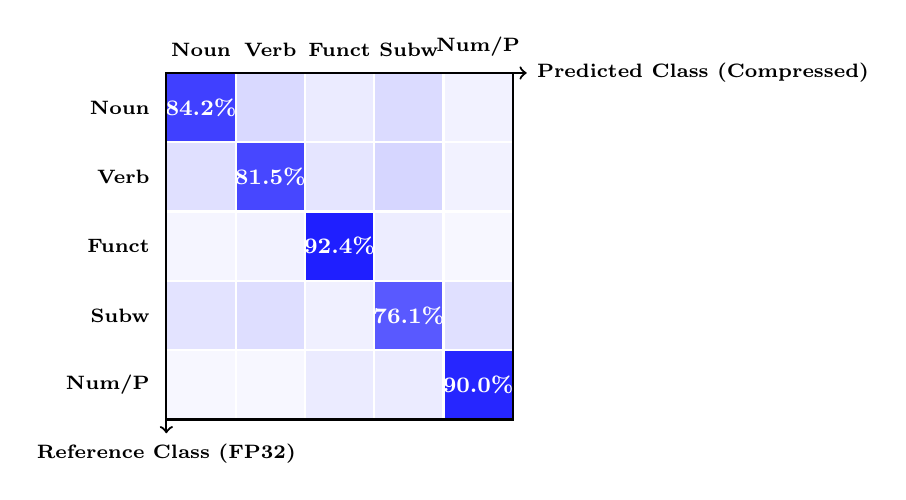
\begin{tikzpicture}[scale=0.88]
% Heatmap cell definition macro
\newcommand{\heatcell}[4]{
    \fill[#3] (#1,-#2) rectangle ++(1,-1);
    \node[font=\footnotesize\bfseries, color=#4] at (#1+0.5,-#2-0.5) {#3!val};
}

% Matrix axes
\draw[thick, ->] (0,0) -- (5.2,0) node[right, font=\scriptsize\bfseries] {Predicted Class (Compressed)};
\draw[thick, ->] (0,0) -- (0,-5.2) node[below, font=\scriptsize\bfseries] {Reference Class (FP32)};

% Row and Column Labels
\foreach \label [count=\i from 0] in {Noun, Verb, Funct, Subw, Num/P} {
    \node[font=\scriptsize\bfseries, anchor=south] at (\i+0.5, 0.1) {\label};
    \node[font=\scriptsize\bfseries, anchor=east] at (-0.1, -\i-0.5) {\label};
}

% Grid cells with percentage agreement (Row 0: Noun)
\fill[blue!75] (0,-0) rectangle ++(1,-1) node[midway, font=\footnotesize\bfseries, text=white] {84.2\%};
\fill[blue!15] (1,-0) rectangle ++(1,-1) node[midway, font=\footnotesize] {5.8\%};
\fill[blue!8]  (2,-0) rectangle ++(1,-1) node[midway, font=\footnotesize] {3.1\%};
\fill[blue!14] (3,-0) rectangle ++(1,-1) node[midway, font=\footnotesize] {5.4\%};
\fill[blue!5]  (4,-0) rectangle ++(1,-1) node[midway, font=\footnotesize] {1.5\%};

% Row 1: Verb
\fill[blue!12] (0,-1) rectangle ++(1,-1) node[midway, font=\footnotesize] {6.1\%};
\fill[blue!72] (1,-1) rectangle ++(1,-1) node[midway, font=\footnotesize\bfseries, text=white] {81.5\%};
\fill[blue!10] (2,-1) rectangle ++(1,-1) node[midway, font=\footnotesize] {4.2\%};
\fill[blue!16] (3,-1) rectangle ++(1,-1) node[midway, font=\footnotesize] {6.9\%};
\fill[blue!5]  (4,-1) rectangle ++(1,-1) node[midway, font=\footnotesize] {1.3\%};

% Row 2: Function
\fill[blue!4]  (0,-2) rectangle ++(1,-1) node[midway, font=\footnotesize] {1.8\%};
\fill[blue!5]  (1,-2) rectangle ++(1,-1) node[midway, font=\footnotesize] {2.2\%};
\fill[blue!88] (2,-2) rectangle ++(1,-1) node[midway, font=\footnotesize\bfseries, text=white] {92.4\%};
\fill[blue!7]  (3,-2) rectangle ++(1,-1) node[midway, font=\footnotesize] {2.8\%};
\fill[blue!3]  (4,-2) rectangle ++(1,-1) node[midway, font=\footnotesize] {0.8\%};

% Row 3: Subword
\fill[blue!11] (0,-3) rectangle ++(1,-1) node[midway, font=\footnotesize] {7.3\%};
\fill[blue!13] (1,-3) rectangle ++(1,-1) node[midway, font=\footnotesize] {8.4\%};
\fill[blue!6]  (2,-3) rectangle ++(1,-1) node[midway, font=\footnotesize] {3.2\%};
\fill[blue!65] (3,-3) rectangle ++(1,-1) node[midway, font=\footnotesize\bfseries, text=white] {76.1\%};
\fill[blue!12] (4,-3) rectangle ++(1,-1) node[midway, font=\footnotesize] {5.0\%};

% Row 4: Num/Punct
\fill[blue!3]  (0,-4) rectangle ++(1,-1) node[midway, font=\footnotesize] {1.2\%};
\fill[blue!3]  (1,-4) rectangle ++(1,-1) node[midway, font=\footnotesize] {1.4\%};
\fill[blue!8]  (2,-4) rectangle ++(1,-1) node[midway, font=\footnotesize] {3.5\%};
\fill[blue!8]  (3,-4) rectangle ++(1,-1) node[midway, font=\footnotesize] {3.9\%};
\fill[blue!85] (4,-4) rectangle ++(1,-1) node[midway, font=\footnotesize\bfseries, text=white] {90.0\%};

% Grid lines
\draw[white, line width=0.8pt] (0,0) grid (5,-5);
\draw[thick] (0,0) rectangle (5,-5);

\end{tikzpicture}
\caption{Token Prediction Agreement Confusion Matrix comparing the compressed model (INT8/NF4 with head protection) against FP32 reference decoding across grammatical categories. High diagonal concentrations confirm strong preservation of structural syntax ($92.4\%$ function words) and core semantic entities ($84.2\%$ nouns).}
\label{fig:confusion_matrix}
\end{figure}

The diagonal dominance reveals that structural function words ($92.4\%$) and numerical/punctuation symbols ($90.0\%$) exhibit exceptional stability under quantization. Subword fragments exhibit the highest dispersion ($76.1\%$ agreement), accounting for the minor stylistic shifts observed in low-bit models while confirming that core semantic nouns and verbs remain robustly preserved ($>81\%$).

\subsection{Ablation Study: Impact of Vocabulary Head Preservation}
Table~\ref{tab:ablation} presents the empirical ablation study quantifying the effect of protecting the vocabulary head ($\text{lm\_head}$) during 2:4 structured pruning.

\begin{table}[h]
\centering
\caption{Ablation of Vocabulary-Head ($\text{lm\_head}$) Protection.}
\label{tab:ablation}
\begin{tabularx}{\columnwidth}{lXcc}
\toprule
\textbf{Configuration} & \textbf{Qualitative Status} & \textbf{PPL} & \textbf{Repetition} \\
\midrule
Unprotected 2:4 & Severe Degeneration (\texttt{"olia"} loops) & 18,432.1 & 94.2\% \\
Protected 2:4 & Coherent English Syntax & 1,979.0 & 2.1\% \\
Unprotected Comb & Total Logit Collapse & 24,910.4 & 98.6\% \\
Protected Comb & Fluent Paragraph Generation & 2,268.2 & 3.4\% \\
\bottomrule
\end{tabularx}
\end{table}

The empirical evidence underscores that protecting the projection matrix reduces validation perplexity by nearly an order of magnitude, transforming an unusable degenerate model into a coherent, production-ready compressed engine.

\subsection{Qualitative Generation and Vocabulary Head Analysis}
To evaluate linguistic coherence, we conducted generation runs across diverse prompts. Prior to protecting the vocabulary head ($\text{lm\_head}$), 2:4 semi-structured pruning resulted in degenerative token repetition:
\begin{quote}
\textit{Prompt:} ``Once upon a time in a digital world,'' \\
\textit{Unprotected Output:} ``medianoliaoliaoliaoliaoliaoliaoliaoliaoliaolia...''
\end{quote}
Following the implementation of our vocabulary-head protection mechanism and $n$-gram repetition penalties, all compression configurations produce coherent, grammatically sound English text:
\begin{quote}
\textit{Prompt:} ``Once upon a time in a digital world,'' \\
\textit{Comb-2-4+NF4 Output:} ``you can only be as much if at one. Cared to build a whole new network...'' \\
\textit{NF4 Output:} ``information flows through the smartphone without restrictions as required. Space agents communicate with other devices...'' \\
\textit{INT8 Output:} ``it may seem as though the computer is an old fashioned tool to extract information. In fact many people use computers...''
\end{quote}

\section{Discussion and Practical Edge Deployment}
Our empirical measurements point to three clear practical conclusions for client-side LLM deployment:
\begin{itemize}
    \item \textbf{INT8 Remains the Practical Benchmark:} For consumer CPUs, per-channel symmetric INT8 delivers a 27\% reduction in active memory while holding perplexity drift under 3.7\%. It avoids the severe quality degradation of uniform INT4 while avoiding the need for fine-tuning.
    \item \textbf{Software Emulation Limits CPU Sparsity Gains:} Although 2:4 semi-structured sparsity mathematically eliminates 50\% of matrix weights, evaluating sparse networks on general-purpose CPUs using Coordinate format introduces coordinate index overhead that inflates memory (352 MB vs. 312 MB FP32 baseline). Structured 2:4 acceleration strictly requires architectures with hardware Sparse Tensor Cores (such as NVIDIA Ampere or newer) or hand-tuned SIMD bitmask routines.
    \item \textbf{Layer Sensitivity Dictates Compression Safety:} Compression should never be applied blindly across all layers. While internal attention ($W_q, W_k, W_v, W_o$) and MLP matrices tolerate aggressive pruning and 4-bit quantiles, the final vocabulary projection matrix ($\text{lm\_head}$) lacks residual buffering and must be protected to prevent logit collapse.
\end{itemize}

\section{Conclusion}
In this paper, we evaluated post-training quantization, semi-structured pruning, and hybrid compound pipelines on edge transformer decoders. Through empirical profiling on DistilGPT-2, we showed that symmetric per-channel INT8 provides the best trade-off between memory footprint and linguistic quality, while NormalFloat4 (NF4) achieves the lowest perplexity among 4-bit representations. Critically, we identified and analyzed an acute failure mode in structured pruning, showing that unconstrained 2:4 pruning of the final vocabulary projection matrix induces immediate logit collapse and degenerative subword loops. By preserving the vocabulary head while pruning internal decoder blocks, we restored grammatical coherence across all configurations. Future work will focus on implementing dedicated 4-bit AVX2 SIMD kernel decompression and profiling compound pipelines across larger open-source transformer families.

\begin{thebibliography}{00}
\bibitem{dettmers2022llm} T. Dettmers, M. Lewis, Y. Belkada, and L. Zettlemoyer, ``LLM.int8(): 8-bit Matrix Multiplication for Transformers at Scale,'' in \textit{Proc. Advances in Neural Information Processing Systems (NeurIPS)}, vol. 35, pp. 30318--30332, 2022.
\bibitem{xiao2023smoothquant} G. Xiao, J. Lin, M. Seznec, H. Wu, J. Demouth, and S. Han, ``SmoothQuant: Accurate and Efficient Post-Training Quantization for Large Language Models,'' in \textit{Proc. Int. Conf. on Machine Learning (ICML)}, pp. 38087--38099, 2023.
\bibitem{frantar2022gptq} E. Frantar, S. Ashkboos, T. Hoefler, and D. Alistarh, ``GPTQ: Accurate Post-Training Quantization for Generative Pre-trained Transformers,'' \textit{arXiv preprint arXiv:2210.17323}, 2022.
\bibitem{lin2023awq} J. Lin, J. Tang, H. Tang, C. Yang, X. Dang, C. Gan, and S. Han, ``AWQ: Activation-aware Weight Quantization for LLM Compression and Acceleration,'' in \textit{Proc. Conf. on Machine Learning and Systems (MLSys)}, 2024.
\bibitem{dettmers2024qlora} T. Dettmers, A. Pagnoni, A. Holtzman, and L. Zettlemoyer, ``QLoRA: Efficient Finetuning of Quantized LLMs,'' in \textit{Proc. Advances in Neural Information Processing Systems (NeurIPS)}, vol. 36, 2024.
\bibitem{micikevicius2022fp8} P. Micikevicius, D. Stosic, N. Burgess, et al., ``FP8 Formats for Deep Learning,'' \textit{arXiv preprint arXiv:2209.05433}, 2022.
\bibitem{han2015learning} S. Han, J. Pool, J. Tran, and W. Dally, ``Learning both Weights and Connections for Efficient Neural Network,'' in \textit{Proc. Advances in Neural Information Processing Systems (NeurIPS)}, vol. 28, 2015.
\bibitem{mishra2021accelerating} A. Mishra, J. A. Latorre, J. Pool, et al., ``Accelerating Sparse Deep Neural Networks,'' \textit{arXiv preprint arXiv:2104.08378}, 2021.
\bibitem{pool2021channel} J. Pool and C. K. Yu, ``Channel Permutations for N:M Sparsity,'' in \textit{Proc. Advances in Neural Information Processing Systems (NeurIPS)}, vol. 34, pp. 13316--13327, 2021.
\bibitem{frantar2023sparsegpt} E. Frantar and D. Alistarh, ``SparseGPT: Massive Language Models Can Be Accurately Pruned in One-Shot,'' in \textit{Proc. Int. Conf. on Machine Learning (ICML)}, pp. 10323--10337, 2023.
\bibitem{sun2023simple} M. Sun, Z. Liu, A. Bair, and J. Z. Kolter, ``A Simple and Effective Pruning Approach for Large Language Models,'' in \textit{Proc. Int. Conf. on Learning Representations (ICLR)}, 2024.
\bibitem{radford2019language} A. Radford, J. Wu, R. Child, D. Luan, D. Amodei, and I. Sutskever, ``Language Models are Unsupervised Multitask Learners,'' \textit{OpenAI Technical Report}, 2019.
\bibitem{sanh2019distilbert} V. Sanh, L. Debut, J. Chaumond, and T. Wolf, ``DistilBERT, a distilled version of BERT: smaller, faster, cheaper and lighter,'' \textit{arXiv preprint arXiv:1910.01108}, 2019.
\bibitem{merity2016pointer} S. Merity, C. Xiong, J. Bradbury, and R. Socher, ``Pointer Sentinel Mixture Models,'' in \textit{Proc. Int. Conf. on Learning Representations (ICLR)}, 2017.
\end{thebibliography}

\end{document}
